% !TeX program = xelatex

\section{Django}
Pyhton bietet 4 große Webframeworks an. Django, Flask, FastAPI und Pyramid. 
Django ist das bekannteste und am weitesten verbreitete Framework. Es ist ein Full-Stack-Framework, 
das viele Funktionen und Bibliotheken mitbringt, um die Entwicklung zu vereinfachen. Flask ist ein Microframework, das nur die grundlegenden Funktionen bietet, ansonsten eigenständig erweitert werden muss.
Pyramid ist ein Framework, das sich in der Mitte dieser beiden Frameworks befindet. Es bietet mehr Funktionen als Flask, ist aber nicht so umfangreich wie Django. 
FastAPI hingegen ist ein neues Framework, welches auf Geschwindigkeit ausgelegt ist. Es ist noch ein recht neues Framework, welches noch in der Entwicklung steckt und daher nicht die Stabilität oder den Umfang anderer besitzt.
Um eine stabile, wartbare und erweiterbare Software zu entwickeln, wurde daher Django als Framework ausgewählt.

\subsection{Django API Architektur}
Die Spring-Boot-Architektur ist von Regeln und Design Patterns geprägt, um flexibel und möglichst generisch agieren zu können. 
Unterstützt durch die objektorientierte Architektur von Java und Spring Injections, ist dies notwendig.

Python hingegen ist keine rein objektorientierte Sprache, sondern eine Skriptsprache, die OOP-Ansätze unterstützt, diese aber nicht erzwingt. 
Eine klare Trennung in Schichten ist hier nicht so einfach und würde oft zu erhöhtem Aufwand und unnötigem Boilerplate-Code führen. In Django werden Aufgaben in eigene Apps unterteilt, 
wobei sich die Aufgaben der Django API grob in drei Bereiche aufspalten lassen. Die Basis für beide Ansätze sind Daten, daher findet der Upload und die Vorverarbeitung von Daten in einer 
"shared" App statt. Dort sind auch die später detaillierter erklärten Imputationsalgorithmen und die Datenvorverarbeitungslogik angesiedelt.

Machine Learning und Time Series Analysis verhalten sich grundsätzlich unterschiedlich und erhalten daher jeweils ihre eigene App, was auch mit verschiedenen URL-Pfaden einhergeht und die Funktionalitäten logisch voneinander trennt.

Innerhalb der Apps wird die Architektur festgelegt. Da Interfaces und Dependency Injection nicht direkt Teil von Django sind und nur über zusätzliche Pakete und Frameworks eingebunden werden können, 
was zusätzliche Komplexität bedeutet, wurde hierauf verzichtet und eine dreischichtige Architektur gewählt. Diese unterteilt sich in Views, Services und Datenbankaktionen. Views sind fachlich äquivalent zu 
Spring-Controllern und definieren daher die REST-Endpunkte, deren Pfade zentral in einem separaten "urls.py" festgelegt werden. Die Services, hauptsächlich für CRUD-Funktionalitäten genutzt, bilden das Logik-Layer ab. 
Sie sind nicht für das Trainieren der ML-Modelle zuständig, da dies über Websockets gesteuert wird, welche separat definiert werden. Im TSA-Bereich kümmert sich ein Endpunkt um die Datenerstellung, 
da diese fast sofort zugänglich sind und kein Websocket benötigt wird.

Um die Logik der Algorithmen von der CRUD-Funktionalität zu trennen, wurden diese in separate Ordner und Strukturen eingebunden. Die Software muss flexibel sein und eine einfache Integration neuer 
Algorithmen ermöglichen. Ein Builder Pattern, das sich einfach erweitern lässt und die Komplexität des Aufbaus eines komplexen Objekts reduziert, bietet sich hierfür an. Es ist durch den Einsatz von 
Default-Implementierungen einfach einsetzbar, ohne neu konfiguriert werden zu müssen. Dieses Konzept funktioniert jedoch nicht im Bereich der verschiedenen Algorithmen. Hier ist es notwendig, sich auf eine 
Basisklasse zu stützen, die gemäß dem OOP-Prinzip bestimmte Funktionalitäten bereitstellt. Alle neuen Algorithmen müssen von dieser Klasse erben und die erforderlichen Funktionen überschreiben oder nutzen.

Im Datenbankdesign existieren die Algorithmen, und ein Strategy Pattern liefert basierend auf der gegebenen Konfiguration den passenden Algorithmus zurück.


\begin{figure}[htbp]
    \centering
\begin{forest}
    for tree={
    font=\ttfamily,
    grow'=0,
    child anchor=west,
    parent anchor=south,
    anchor=west,
    calign=first,
    edge path={
            \noexpand\path [draw, \forestoption{edge}]
            (!u.south west) +(7.5pt,0) |- node[fill,inner sep=1.25pt] {} (.child anchor)\forestoption{edge label};
        },
    before typesetting nodes={
            if n=1
                {insert before={[,phantom]}}
                {}
        },
    fit=band,
    before computing xy={l=15pt},
    }
    [project
        [djangoproject
                [common]
                [settings.py]
                [urls.py]
        ]
        [mlAPI
                [urls.py]
                [mlalgorithms]
                [services]
                [views]
        ]
        [shared 
            [...]
        ]
        [tsaAPI]
    ]
\end{forest}
\caption{Django Projekt Aufbau}
\end{figure}


\subsection{Absicherung der Anwendung über Djangos Sicherheitskonzept}
Wie bereits in Sektion \ref{sec:javaSpringSecurityConfig} beschrieben, wurde für das Projekt eine JWT-Authentifizierung ausgewählt, um einerseits Nutzer zu verifizieren und andererseits die Daten an Nutzerkonten zu binden.
%TODO: Eine bessere Einleitung könnte noch ergänzt werden.

Django bietet hierfür eine Django-JWT-Library an, die nach einem Spring-ähnlichen Konzept funktioniert, indem eine Middleware eingesetzt wird, die die Validierung gleich zu Beginn durchführt. Hierbei traten jedoch zwei Probleme auf. 
Sowohl Spring als auch Django basieren ihre Authentifizierung auf einem Nutzer-Modell. Die Struktur des Django-Nutzermodells ist allerdings nicht direkt kompatibel mit dem, was Spring verwendet. 
Beide Modelle haben unterschiedliche Felder und sind somit nicht direkt miteinander kompatibel.

Es gibt zwei mögliche Lösungen: Einerseits könnte man auf die normalen Nutzermodelle beider Frameworks setzen. Hierbei müssten weder die Modelle angepasst werden noch die Login- bzw. Passwortvalidierung überschrieben werden. 
Zudem wären beide APIs stärker separiert und somit weniger voneinander abhängig. Nachteilig wäre allerdings die doppelte Nutzerverwaltung und der doppelte Anmeldeprozess. Obwohl dieser durch das Frontend abstrahiert werden könnte, 
bleibt die Lösung suboptimal. Eine Option wie OAuth2 wurde ebenfalls verworfen, sodass nur die Anpassung der Modelle als Lösung verbleibt.

Dabei traten einige Probleme auf. Spring und Django unterscheiden sich in der Art und Weise der Nutzer- und Passwortvalidierung und setzen auf unterschiedliche Verschlüsselungsalgorithmen. Da die Priorität der Spring-API höher ist und die Django-API lediglich die Funktionalität der Spring-API erweitert, muss sich die Django-API nach den Vorgaben von Spring richten.

Um Nutzer in Django ähnlich wie in Spring an Methoden binden zu können, wurde ein ähnliches Modell verwendet. Python besitzt zwar kein direktes AOP-Modell, verfügt jedoch über ein ähnliches Interceptor-System.

\begin{lstlisting}[language=Python, caption={Annotation basiertes Anbinden eines Nutzermodelles an eine Methode}, label={code:djangoSecurity}]
def jwt_authenticated(view_func):
    @wraps(view_func)
    def _wrapped_view(request, *args, **kwargs):
        if not request.user.is_authenticated:
            return Response({'detail': 'Authentication credentials were not provided.'},
                            status=status.HTTP_403_FORBIDDEN)
        return view_func(request, request.user, *args, **kwargs)

    return _wrapped_view
\end{lstlisting}

Wie in Listing \ref{code:djangoSecurity} ersichtlich, fängt dieser Interceptor den Methodenaufruf ab und prüft, ob der Nutzer authentifiziert ist. Ist dies nicht der Fall, wird der Request abgewiesen. Andernfalls wird der Nutzer als Argument an die 
Methode angehängt und ist somit im Code verwendbar.

Dieses Modell ist nicht ideal, da der Nutzer bereits am Controller (oder View) angebunden ist und durch die verschiedenen Schichten weitergereicht werden muss. Daher kann er nicht einfach ersetzt oder ausgetauscht werden, ohne signifikante Teile des Codes 
zu verändern. Eine Alternative wäre die Nutzung eines thread-local Stores, um den Nutzer wieder in den DatenbankService zu verlagern und somit vom Business-Code zu trennen, wodurch er einfacher veränderbar wäre. Dieser Ansatz wurde zwar ausprobiert, 
erwies sich jedoch nicht als stabil genug und wurde letztendlich verworfen.

Im Django-Datenmodell hängen nicht alle Elemente an einem zentralen Punkt, wie es beispielsweise in der Spring-API der Fall ist. Hier ist der Nutzer nur an bestimmten Entitäten angebunden. Die grundlegenden Modelle im Bereich Machine Learning oder 
Time Series Analysis sind unabhängig vom Nutzer und stehen jedem zur Verfügung. Die hochgeladenen Daten und die Konfigurationen, die aus den Daten erstellt werden und später auch in Spring genutzt werden sollen, sind jedoch stark nutzerabhängig und sollten 
dementsprechend auch nur von ihm abrufbar sein.


\subsection{Bidirektionale Kommunikation über Django Channels}
Maschinelles Lernen ist ein sehr rechen- und zeitintensiver Prozess, der im klassischen Call-Response-Prinzip von \ac{REST} schlecht aufgehoben ist. Nutzer reagieren, besonders im \ac{UI}-Umfeld, sehr sensibel auf 
Verzögerungen und fehlendes visuelles Feedback. Es ist wichtig, dass Nutzer sehen können, dass etwas passiert, und sie sollten daher auch über den aktuellen Fortschritt informiert werden.

Die sinnvollste Lösung für dieses Problem ist die Nutzung eines Websockets, der an die Callbacks der Modelle gebunden wird und somit den Nutzer über den aktuellen Fortschritt informiert. 
Django unterstützt Websockets\footcite{https://channels.readthedocs.io/en/latest/} nicht direkt, weshalb hier auf das Framework Channels zurückgegriffen wurde. Channels integriert Websockets 
in Django und bietet somit die Möglichkeit, diese zu nutzen. Channels basiert auf Redis und verwendet es als Message Broker. Redis, wie bereits in \ref{sec:redis} erwähnt, ist eine In-Memory-Datenbank, 
die aufgrund ihrer Schnelligkeit gut für die Kommunikation zwischen Threads geeignet ist.


\begin{lstlisting}[language=Python, caption={Websocket Konsumer}, label={code:djangoWebsocket}]
    class StatusConsumer(JsonWebsocketConsumer):
    runners = {}

    def connect(self):
        group_name = f"model{self.scope['ml_id']}solution{self.scope['sol_id']}"
        try:
            async_to_sync(self.channel_layer.group_add)(group_name, self.channel_name)
            self.scope["group"] = group_name
            self.accept()
        except Exception as e:
            logging.error(e)
            raise UnknownErrorException("cannot connect", reason=str(e))

    def disconnect(self, close_code):
        async_to_sync(self.channel_layer.group_discard)
            (self.scope["group"], self.channel_name)

    def receive_json(self, message, **kwargs):
        response = self.prepare_data(message)
        self.send_json(response)

    def chat_message(self, event):
        self.send_json(event["message"])

    def chat_disconnect(self, event):
        self.send_json(event["message"])
        self.close()
        self.runners.get(event["uuid"])
\end{lstlisting}

Der Code in Listing \ref{code:djangoWebsocket} präsentiert einen JSON-Konsumer, der eine WebSocket-Anfrage annimmt und eine Verbindung aufbaut. Aus der initialen 
Anfrage werden die trainingsrelevanten Informationen extrahiert und an die entsprechende Stelle im Prozess weitergeleitet.

Nachdem die Modelle trainiert worden sind, wird der finale Status an den Nutzer gesendet und anschließend die Verbindung getrennt.

\subsection{Fehlerbehandlung und Verarbeitung}
Das System implementiert ebenfalls ein interceptor-basiertes Error-Handling nach dem "Fail-Fast"-Prinzip. Illegale Optionen, invalide Parameter und ungültige Dateitypen führen zum Auslösen einer 
Exception, die von speziell dafür vorgesehenen Exception-Handlern abgefangen und verarbeitet wird. Auch hier wurde ein Format gewählt, das der Spring-Variante ähnelt, um ein kohärentes und einheitliches 
Fehlermeldungsprinzip zu gewährleisten.

\begin{lstlisting}[language=Python, caption={Exception Handler}, label={code:djangExceptionHandler}]
def exception_handler(exc, context):
    def build_error_response(exception, status_code):
        response_data = {
            "error": str(exception),
            "reason": exception.reason if hasattr(exception, 'reason') else None,
            "i18nKey": exception.i18nKey if hasattr(exception, 'i18nKey') else "UNDEFINED"
        }
        return JsonResponse(response_data, status=status_code)

    exception_mapping = {
        NotFoundException: status.HTTP_404_NOT_FOUND,
        BadRequestException: status.HTTP_400_BAD_REQUEST,
        InvalidFileTypeException: status.HTTP_400_BAD_REQUEST,
        UnknownErrorException: status.HTTP_500_INTERNAL_SERVER_ERROR,
        UniqueConstraintViolationException: status.HTTP_409_CONFLICT,
        UserNotAuthenticated: status.HTTP_403_FORBIDDEN
    }

    if type(exc) in exception_mapping:
        return build_error_response(exc, exception_mapping[type(exc)])

    if isinstance(exc, UnknownErrorException):
        logging.error(f"unknown error: {exc}")

    response = drf_exception_handler(exc, context)
    if response is not None:
        return response

    return JsonResponse({'error': 'Unexpected server error'}, 
        status=status.HTTP_500_INTERNAL_SERVER_ERROR)
\end{lstlisting}

Die in Listing \ref{code:djangExceptionHandler} dargestellte Exception Map ermöglicht es, selbst definierte Exceptions auf einen \ac{REST} Error Code zu projizieren. Dadurch ist sie flexibel in der Nutzung und leicht anpassbar.


\subsection{Validierung der Daten und Vorverarbeitung}
\label{sec:djangoDataPreprocessing}
Es ist nicht davon auszugehen, dass alle Daten in einer homogenen Form vorliegen und normalisiert sind. Dies stellt jedoch eine grundlegende Anforderung dar, nicht nur um die Modelle effektiv konstruieren zu können, sondern auch um ...

\paragraph*{Fehlende Werte im Datensatz}
Die Handhabung von Daten in Zeitreihen stellt eine besondere Herausforderung dar, insbesondere wenn nicht sichergestellt ist, dass die Daten immer im gleichen Abstand aufgezeichnet oder mit Zeitstempeln versehen wurden. Unter diesen Bedingungen wurde ein Algorithmus entwickelt, der die Struktur der Daten erkennt, sie entsprechend kategorisiert oder umwandelt und in ein uniformes Format überführt.

Angesichts der Komplexität, die mit der Unterstützung verschiedener Dateiformate einhergeht, wurden einige Annahmen getroffen:
\begin{enumerate}
    \item Bei mehreren unbenannten Datensätzen in einer Datei wird geprüft, ob eine dieser Zeitreihen konsequent linear ansteigt. Ist dies der Fall, werden diese Werte als Zeitstempel interpretiert.
    \item Ist keine konsequent steigende Zeitreihe zu finden, wird den Daten ein normaler Anstieg zugeordnet.
    \item Dateiformate wie JSON oder CSV, die Header oder Dictionaries nutzen, erfordern eine spezielle Taxonomie, um die Zeitreihe im Dokument zu identifizieren, die für die Zeiterfassung gedacht ist. Wenn eine solche gefunden wird, wird sie jeder Zeitreihe hinzugefügt.
\end{enumerate}

Basierend auf diesen Annahmen wurde ein Algorithmus entwickelt, abhängig vom Datenformat. Dieser durchsucht die Datei, testet auf mögliche Strukturen und bearbeitet sie anschließend, wie in Abbildung \ref{fig:upload_data} dargestellt.

\begin{figure}[h]
    \centering
    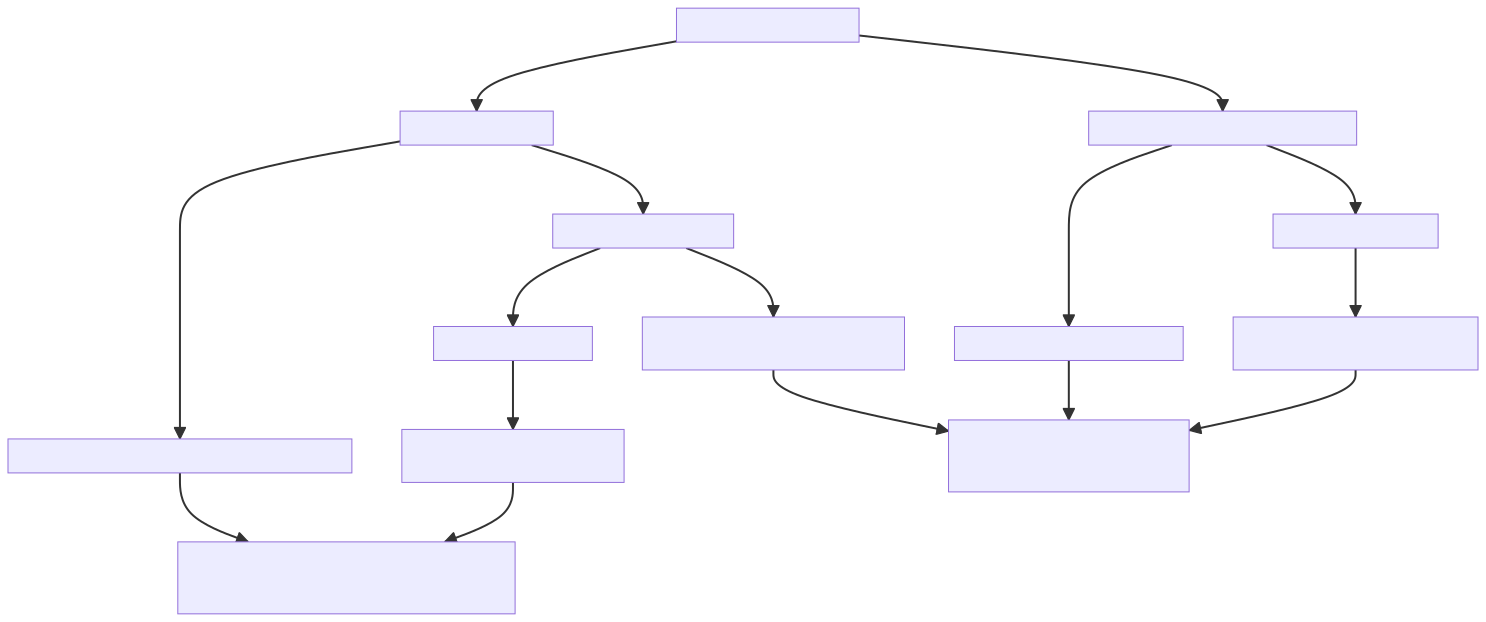
\includegraphics[width=0.9\linewidth]{includes/figures/upload_process.png}
    \caption{Algorithmus zum zerlegen einer hochgeladenen JSON Datei}
\label{fig:upload_data}
\end{figure}



Diese Vorverarbeitung der Daten erfolgt bereits beim Hochladen und stellt sicher, dass die Daten im weiteren Verlauf immer in einem uniformen Format vorliegen. 
Die Überprüfung der Daten auf Lücken wird erst bei Bedarf durchgeführt. Da nur die Zeitstempel eine Rolle spielen und diese im Unix-Format vorliegen, berechnet der Algorithmus die Differenz aufeinanderfolgender Werte. Hierbei wird ein Schwellenwert definiert, um kleine Ungenauigkeiten zu ignorieren. Bei signifikanten Abweichungen von der Standarddistanz wird eine Lücke angenommen.

Der Algorithmus zum Identifizieren und Füllen von Lücken ist in Listing \ref{enum:django_gap_handling} zu finden. Er beschreibt, wie Lücken nach bestimmten Kriterien 

definiert werden und zeigt auf, wie diese geschlossen werden. In diesem Schritt werden die Lücken noch nicht klassifiziert oder gefüllt, sondern lediglich mit \textit{NaN}-Werten markiert. Dadurch entsteht eine Zeitreihe, in der alle Werte in regelmäßigen Abständen vorhanden sind.

\begin{lstlisting}[language=Python, caption={Algorithmus zum Auffüllen von Lücken}, label={code:djangoAlgoGap}]
def __find_differences_in_steps_and_fill_them_with_nan(train_data, timestamps_normalized):
    processed_train_data = []
    processed_time_stamps = []
    for i, (train_d, timestamp_d) in enumerate(zip(train_data, timestamps_normalized)):
        differences = np.diff(timestamp_d)
        threshold = differences.min() + differences.min() * error_percentage
        large_gap_indices = np.where(differences > threshold)[0]
        start_gap = large_gap_indices
        end_gap = large_gap_indices + 1
        diff = np.ceil(-(differences[end_gap] - differences[start_gap]) / threshold)
        new_timestamps = np.copy(timestamp_d)
        new_train_d = np.copy(train_d)
        for index, size in sorted(zip(end_gap, diff), key=lambda x: x[0], reverse=True):
            nan_array = np.full(int(np.round(size)), np.nan)
            new_timestamps = np.insert(new_timestamps, index, nan_array)
            new_train_d = np.insert(new_train_d, index, nan_array)
        processed_train_data.append(new_train_d)
        processed_time_stamps.append(new_timestamps)
    return processed_train_data, processed_time_stamps
\end{lstlisting}

Für das Füllen von Lücken wurden unterschiedliche Ansätze abhängig von der Größe der Lücke gewählt. Kleine Lücken werden durch Imputationsalgorithmen gefüllt, indem die umgebenden Werte herangezogen werden, um die wahrscheinlichsten Ersatzwerte zu ermitteln. 
Es wurden verschiedene Algorithmen implementiert, zwischen denen der Nutzer per Eingabe im Frontend wählen kann. Diese Algorithmen werden als Funktion übergeben, erhalten die relevanten Daten und liefern die aufgefüllte Version zurück. Dies ermöglicht ein sehr 
flexibles Vorgehen und kann daher auch ohne großen Aufwand erweitert werden. Bei größeren Lücken, wo der Informationsverlust zu groß wäre, bleiben die Werte leer und erhalten den in Python üblichen \textit{NaN}-Wert (Not a number). Die Handhabung dieser leeren Werte obliegt den nachfolgenden Algorithmen, die in den Sektionen \ref{sec:djangoML} und \ref{sec:djangoTSA} näher erläutert werden.

\paragraph{Uniformisierung der Daten}
Eine uniforme Version der Daten ist besonders wichtig im Bereich des maschinellen Lernens, da Trainingsdaten in unterschiedlichen Längen und Bereichen (beispielsweise von 0 bis 1) die Ergebnisse verfälschen oder das Training erschweren können. Daher ist es notwendig, die Daten zu normalisieren und auf eine einheitliche Länge zu bringen. 
Oft ist auch eine Reduzierung oder Komprimierung der Daten sinnvoll. Zwar gehen dabei Informationen verloren, aber da die Grundstruktur des Datensatzes erhalten bleibt und die Performance des Modells 
deutlich erhöht wird, sollte diese Option den Nutzern angeboten werden. Teilweise ist dies auch notwendig, da Modelle ab einer gewissen Größe nicht mehr auf jeder Hardware laufen.

Den Nutzern werden viele Möglichkeiten gegeben, selbstständig die Komprimierung vorzunehmen und eventuell lineare Trends aus den Daten zu entfernen. Weitere Optionen können problemlos hinzugefügt werden, da dafür lediglich ein JSON-Schema, die Implementierung sowie die Integration in das Strategy Pattern notwendig sind. Alle Änderungen im Vorverarbeitungsschritt werden in der Datenbank gespeichert und sind umkehrbar, sodass beim späteren Versenden der Daten diese wieder in der Form vorliegen, in der die Originaldaten hochgeladen wurden. Die verschiedenen Implementierungen werden über ein Strategy Pattern gezielt angesprochen und über JSON-Dictionaries mit ihrer spezifischen Konfiguration geladen.



\subsection{Generalisierung und Nutzung der Machine Learning Modelle}
\label{sec:djangoML}
Python ist eine der führenden Sprachen im Bereich des maschinellen Lernens und bietet daher eine umfangreiche Auswahl an Bibliotheken und Frameworks, die mit hilfreichen Komponenten und Funktionen ausgestattet sind. 
Große Frameworks wie TensorFlow oder PyTorch bieten zahlreiche Möglichkeiten, sind jedoch auch sehr komplex und erfordern viel Zeit, um gewünschte Modelle zu entwickeln. Aus diesem Grund wurde in diesem Projekt auf Keras gesetzt, 
das eine Abstraktionsebene über TensorFlow bietet und somit die Komplexität reduziert. Keras ermöglicht das Erstellen von Modellen über ein \ac{ANN}, die sich durch die Konfiguration der Schichten und Neuronen anpassen lassen.

Wie im Kapitel \ref{cha:stateOfTheArt} ersichtlich, sind \acp{GAN} und \acp{RNN} verbreitete Ansätze, um aus einer Menge von Trainingsdaten synthetische Daten zu generieren. Da ein Ziel dieser Arbeit der Vergleich dieser Ansätze ist, 
wurden verschiedene Modelle beider Varianten implementiert.

In der Praxis unterscheidet die Django-API nicht zwischen den beiden Varianten, da beide über dasselbe Interface angesprochen werden. Das zugrundeliegende Strategy Pattern liefert die passende Implementierung.


\begin{lstlisting}[language=Python, caption={Grundklasse zum Trainieren der Machine Learning Modelle, sie stellt Grundmethoden und geteilte Funktionalitäten bereit}, label={code:djangoAlgoGAN}]    
class GeneralMLModel:
    data: List[np.ndarray] = None
    run_information: RunInformation = None

    def set_config(self, config: RunInformation):
        """ set configuration for model """
        pass

    def set_data(self, data: List[np.ndarray]):
        """ set data for model """
        pass

    def run(self):
        """ start training the model  """
        pass

    def predict_data_from_model(self):
        """ predict data from model """
        pass

    def forcast(self, limit: int, starting_point: int = -1) -> np.array:
        """ forcast data from model, does not work for every model """
        pass

    def save(self, model: Model) -> RunInformation:
        """ write model to file and save base64 string in database """
        pass

    def load_model(self) -> Model:
        """ write model from database to file and load it from there """
        pass

    def create_image(self, real: List[np.array], synthetic: List[np.array], title: str):
        """ create an image and save it as base64 string """
        pass
\end{lstlisting}

\paragraph{Generative Modelle}
\label{sec:djangoGAN}
Zwei funktionierende \acp{GAN} wurden implementiert: das normale \ac{GAN} und das \ac{CGAN}. Mit \acp{WGAN} und \acp{TGAN} wurde ebenfalls experimentiert, und es existieren Testversionen dieser im Testframework (siehe Abschnitt \ref{sec:tested_models}). 
Da diese jedoch nicht die gewünschten Ergebnisse lieferten, stehen sie momentan nur in der Entwicklungsumgebung zur Verfügung und werden nicht von der API angeboten. Beide implementierten Varianten umfassen einen Generator und einen Diskriminator, 
wobei die Eingabedimensionen von der Länge der zu trainierenden Zeitreihe abhängen. Daher spielt die Normalisierung der Daten eine entscheidende Rolle, um Übereinstimmungen in den Dimensionen der Schichten zu gewährleisten.

\paragraph{Rekursive Modelle}
\acp{RNN} analysieren Daten in ihrer zeitlichen Abfolge und eignen sich daher besonders gut für die Analyse oder Vorhersage von Zeitreihen. Die von ihnen generierten Daten sind stark abhängig von der Variabilität der Trainingsdaten. 
Da sie jedoch in der Lage sind, Vorhersagen über künftige Verläufe zu erstellen, bieten sie Möglichkeiten, die generative Modelle nicht bieten. Deshalb wurden sie in das System integriert. Die Auswahl der Parameter erfolgt allerdings erst in der Spring-API, 
da dort die entsprechenden Datensätze erstellt und die JSON-Schemata mit den dazugehörigen Regeln definiert werden.

\paragraph{Abhängigkeitsprobleme}
Ein wesentliches Problem stellte die Integration weiterer Modelle aus verschiedenen Bibliotheken dar. Viele Bibliotheken befassen sich mit Datengenerierung, sind jedoch untereinander nicht immer kompatibel, was zu Abhängigkeitskonflikten führte. 
Dies verhinderte die direkte Nutzung dieser Bibliotheken.

\subsection{Generalisierung und Nutzung der Zeitreihenanalysealgorithem}
\label{sec:djangoTSA}

Die Zeitreihenanalyse ist der zweite Hauptansatz zur Generierung von Daten. Dabei werden die Daten in ihre Bestandteile zerlegt, um Muster zu erkennen und diese zu nutzen, um neue Daten zu generieren. 
Wie bereits in Kapitel \ref{cha:stateOfTheArt} beschrieben, gibt es verschiedene Ansätze für die Zeitreihenanalyse, die sich in ihrer Komplexität und ihren Ergebnissen unterscheiden.

Zwei vielversprechende Ansätze in diesem Bereich sind die Singular Spectrum Analysis (\ac{SSA}) und die Empirical Mode Decomposition (\ac{EMD}). Diese Methoden zielen darauf ab, Muster in den Daten durch die Zerlegung in 
(\acp{IMF}) zu identifizieren und für die Generierung neuer Daten zu nutzen. Die Implementierung dieser Algorithmen ist zwar rechenintensiv, aber im Vergleich zu maschinellen Lernansätzen nicht so aufwendig, da sie nicht trainiert werden 
müssen und nur einmalig ausgeführt werden. Python bietet bereits Bibliotheken, die diese Algorithmen implementieren. Daher besteht die Herausforderung hauptsächlich darin, die Daten in das richtige Format zu bringen und dem Nutzer Zugriff auf die 
generierten Daten zu gewähren.

Obwohl dieser Ansatz in der Testphase nicht berücksichtigt wurde, bietet die Zerlegung der Daten in ihre Bestandteile einen weiteren interessanten Vorteil für den Nutzer. Da die Daten dem Nutzer grafisch dargestellt werden, 
kann er selbst Muster erkennen und diese nach Belieben verschieben. Dies ermöglicht es ihm, die Ausgangsdaten zu manipulieren und zu verändern, um so neue Daten zu generieren. Der Nutzer behält somit die Kontrolle 
und überlässt sie nicht nur dem Algorithmus. Weitere Details dazu werden im Kapitel \ref{sec:reactTSA} erläutert.

Um weitere Ansätze zu testen und anzubieten, wurden auch klassische Methoden wie die Amplitude Modulation and Noise (AMIRA) und der Cubic Spline Algorithmus implementiert. Diese Methoden interpolieren die Daten und bieten 


somit eine andere Form der Datenabstraktion. Beide Methoden sind sehr schnell und liefern gute Ergebnisse. Allerdings sind sie nicht in der Lage, neue Daten zu generieren, da sie lediglich die vorhandenen Daten interpolieren und nicht nach Mustern suchen.

Die Integration dieser Algorithmen in die API erfolgt ähnlich wie im Kapitel \ref{sec:djangoML} und sie sind ebenfalls über ein Strategiemuster auswählbar.



\subsection{Das Datenbank Modell}

Aus den in den vorherigen Sektionen beschriebenen Anforderungen an die Datenstruktur wurde ein Datenbankmodell entwickelt, das die Anforderungen erfüllt und gleichzeitig flexibel genug ist, um die Erstellung komplexer Simulationsumgebungen zu ermöglichen.
Dieses ist in Abbildung \ref{fig:datamodel_new_version} dargestellt und zeigt den aktuellen Stand der finalen Software.

\begin{figure}[ht]
    \centering
    \includegraphics[width=1\textwidth]{includes/figures/database/software.png}
    \caption{Entity-Relationship-Diagramm der aktuellen Datenstruktur}
    \label{fig:datamodel_new_version}
\end{figure}

Wie in dem Bild zu sehen ist, dient der Nutzer als zentraler Punkt und besitzt viele verschiedene Entitäten, die mit ihm verknüpft sind. Wichtig sind hiervorallem die TrainingData, welche die hochgeladenen Daten beinhalten, die Projects, welche seine Projekte aufspannen, und die jeweiligen Konfigurationen für \ac{ML} und \ac{TSA} Modelle.
Die ausenstehenden Entitäten der Schemata sind für die flexibele Zusammensetzung der jeweiligen JSON-Schemata notwendig.
